% Chapter Template

\chapter{FDTD - Three-Dimensional Scenario} % Main chapter title

\label{Chapter4} % Change X to a consecutive number; for referencing this chapter elsewhere, use \ref{ChapterX}

%----------------------------------------------------------------------------------------
%	SECTION 1
%----------------------------------------------------------------------------------------

\section{Main Section 1}


%-----------------------------------
%	SUBSECTION 1
%-----------------------------------
\subsection{Subsection 1}


%-----------------------------------
%	SUBSECTION 2
%-----------------------------------

\subsection{Subsection 2}

%----------------------------------------------------------------------------------------
%	SECTION 2
%----------------------------------------------------------------------------------------

\section{C++ Implementation}

\begin{minted}[breaklines,frame=single]{c++}
const double permitivity = 8.854e-12;
const double permeability = 1.256e-6;

double L = 5;
int N = 50;
int iterNum = 200;
double deltaX = L / N;
double deltaY = L / N;
double deltaZ = L / N;
double deltaT = (deltaZ * sqrt(permitivity*permeability)  * (1/sqrt(3))); // 1/C * 1/sqrt2 * deltaZ

// variables needed for Gaussian Pulse excitation
double eps = 1e-3;
double Teps = 50 * deltaT;
double beta = -(pow((2/Teps), 2) * log(eps));


vector<vector<vector<double>>> Ex(N, vector<vector<double>>(N, vector<double>(N, 0)));
vector<vector<vector<double>>> Ey(N, vector<vector<double>>(N, vector<double>(N, 0)));
vector<vector<vector<double>>> Ez(N, vector<vector<double>>(N, vector<double>(N, 0)));
vector<vector<vector<double>>> Hx(N, vector<vector<double>>(N, vector<double>(N, 0)));
vector<vector<vector<double>>> Hy(N, vector<vector<double>>(N, vector<double>(N, 0)));
vector<vector<vector<double>>> Hz(N, vector<vector<double>>(N, vector<double>(N, 0)));

const string filePath = "./Out/";

void writeDataToCsvFile(string filename, vector<vector<vector<double>>> Vx, vector<vector<vector<double>>> Vy, vector<vector<vector<double>>> Vz){
	ofstream csvFile(filename);
	csvFile << "x,y,z,Vx,Vy,Vz\n";
	
	for (unsigned  x = 0; x < Vx[0][0].size(); x++) {
		for (unsigned  y = 0; y < Vy[x][0].size(); y++) {
			for (unsigned  z = 0; z < Vz[x][y].size(); z++) {
				csvFile << x << "," << y << "," << z << "," << Vx[x][y][z] << "," << Vy[x][y][z] << "," << Vz[x][y][z] << "\n";
			}
		}
	}
	
	csvFile.close();
}

int main()
{
  for(int i = 0; i < iterNum; i++) {
		
		double t = i * deltaT;
		double gamma = Teps / 2;
		
		// reducing the magnitude since in free space
		Ex[24][24][24] = exp(-(beta * pow((t - gamma), 2))) * 10e-4;  //TO-DO: Gaussian excitation, alpha = 1, Teps = 50*deltaT, eps = 1e-3, t = i * deltaT
		//Ey[9][9][9] = exp(-(beta * pow((t - gamma), 2))) * 10e-4;
		//Ez[9][9][9] = exp(-(beta * pow((t - gamma), 2))) * 10e-4;
		
		// loop for values
		for (int i = 0; i < N-1; i++) {
			for (int j = 0; j < N-2; j++) {
				for (int k = 0; k < N-2; k++) {
					Hx[i][j][k] = Hx[i][j][k] + (deltaT / permeability / deltaZ) * (Ey[i][j][k+1] - Ey[i][j][k] - Ez[i][j+1][k] + Ez[i][j][k]);
				}
			}
		}
		
		for (int i = 0; i < N-2; i++) {
			for (int j = 0; j < N-1; j++) {
				for (int k = 0; k < N-2; k++) {
					Hy[i][j][k] = Hy[i][j][k] + (deltaT / permeability / deltaZ) * (Ez[i+1][j][k] - Ez[i][j][k] - Ex[i][j][k+1] + Ex[i][j][k]);
				}
			}
		}
		
		for (int i = 0; i < N-2; i++) {
			for (int j = 0; j < N-2; j++) {
				for (int k = 0; k < N-1; k++) {
					Hz[i][j][k] = Hz[i][j][k] + (deltaT / permeability / deltaZ) * (Ex[i][j+1][k] - Ex[i][j][k] - Ey[i+1][j][k] + Ey[i][j][k]);
				}
			}
		}
		
		writeDataToCsvFile((filePath + "H/H.csv." + to_string(i)), Hx, Hy, Hz);
		
		for (int i = 0; i < N-2; i++) {
			for (int j = 1; j < N-2; j++) {
				for (int k = 1; k < N-2; k++) {
					Ex[i][j][k] = Ex[i][j][k] + (deltaT / permitivity / deltaZ) * (Hz[i][j][k] - Hz[i][j-1][k] - Hy[i][j][k] + Hy[i][j][k-1]);
				}
			}
		}
		
		for (int i = 1; i < N-2; i++) {
			for (int j = 0; j < N-2; j++) {
				for (int k = 1; k < N-2; k++) {
					Ey[i][j][k] = Ey[i][j][k] + (deltaT / permitivity / deltaZ) * (Hx[i][j][k] - Hx[i][j][k-1] - Hz[i][j][k] + Hz[i-1][j][k]);
				}
			}
		}
		
		for (int i = 1; i < N-2; i++) {
			for (int j = 1; j < N-2; j++) {
				for (int k = 0; k < N-2; k++) {
					Ez[i][j][k] = Ez[i][j][k] + (deltaT / permitivity / deltaZ) * (Hy[i][j][k] - Hy[i-1][j][k] - Hx[i][j][k] + Hx[i][j-1][k]);
				}
			}
		}
		
		writeDataToCsvFile((filePath + "E/E.csv." + to_string(i)), Ex, Ey, Ez);
	}
}
\end{minted}

\section{Data Visualization}

\begin{figure}[h!]
	\centering
	\begin{subfigure}{.49\textwidth}
		\centering
		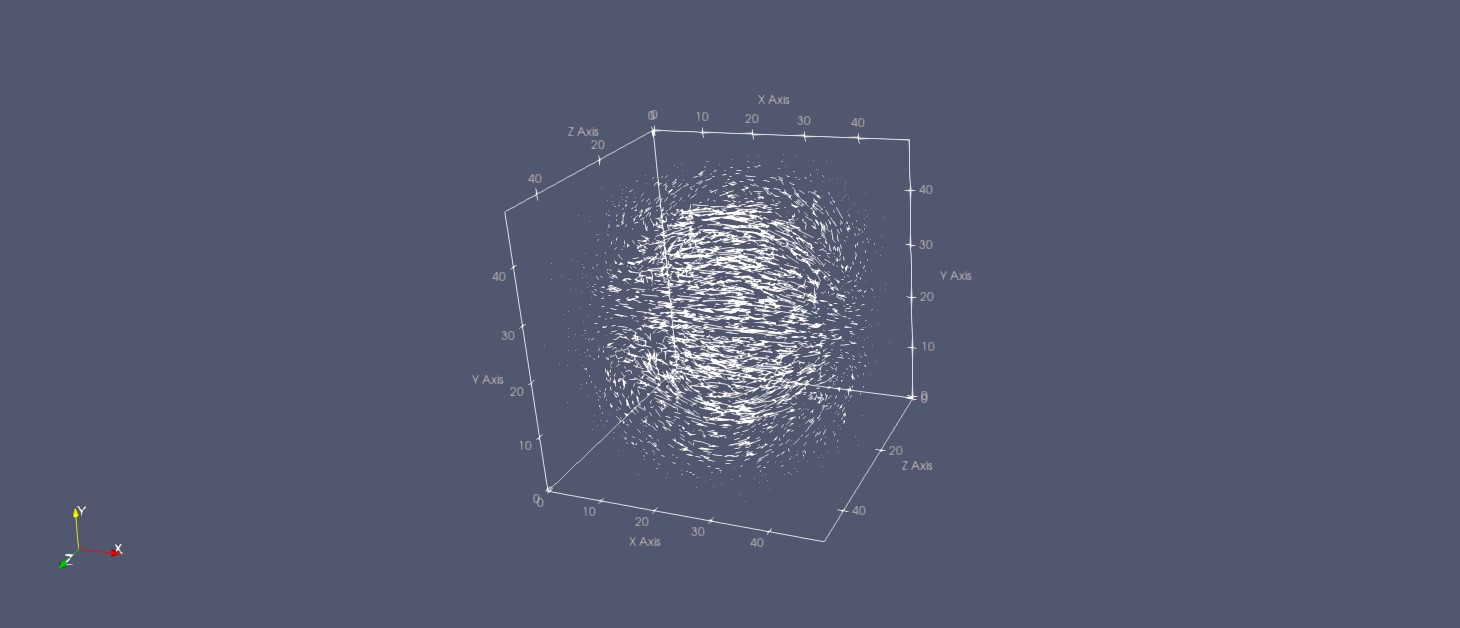
\includegraphics[width=.95\linewidth]{Figures/FDTD3DE1}
		\caption{t = 200}
	\end{subfigure}
	\begin{subfigure}{.49\textwidth}
		\centering
		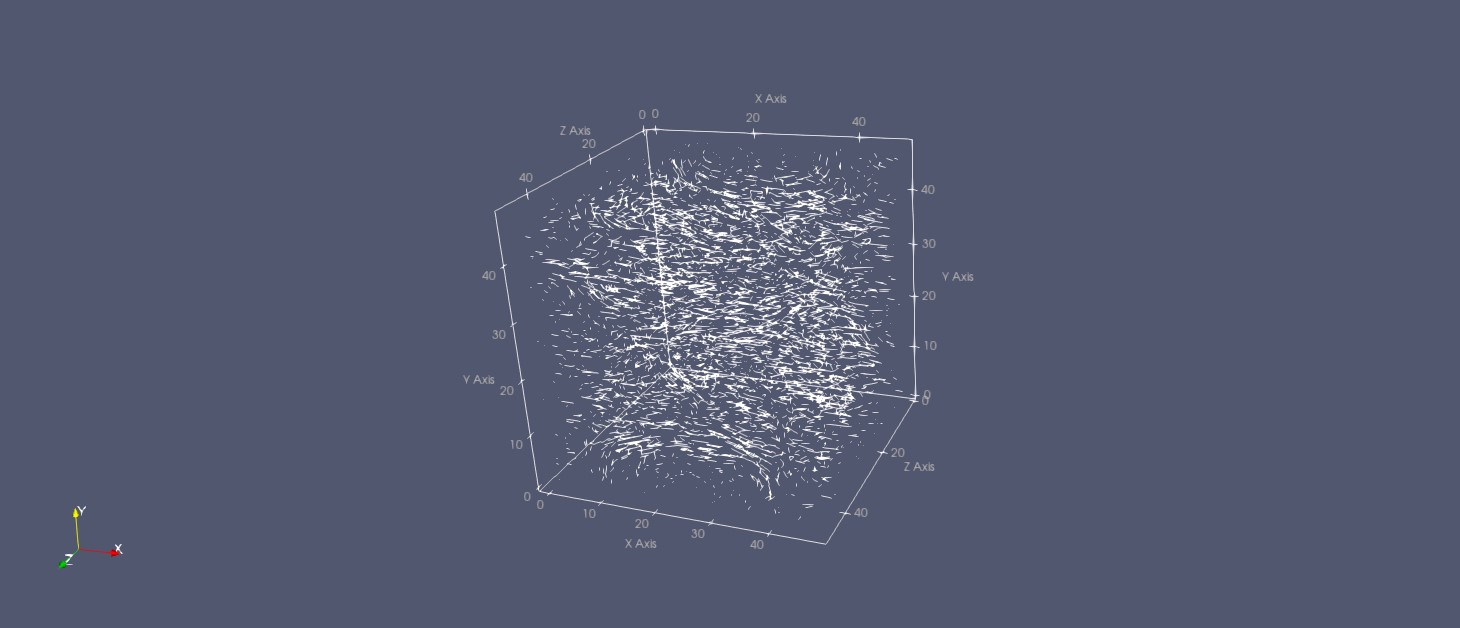
\includegraphics[width=.95\linewidth]{Figures/FDTD3DE2}
		\caption{t = 400}
	\end{subfigure}
	\begin{subfigure}{.49\textwidth}
		\centering
		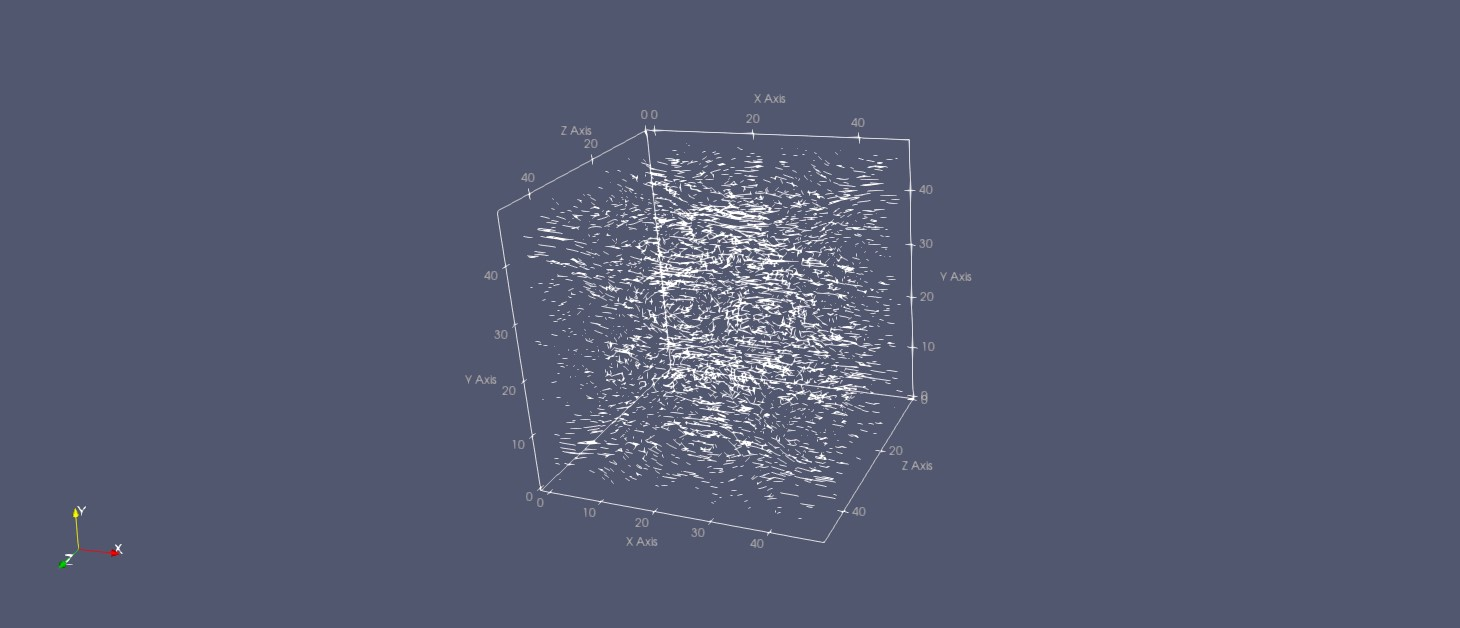
\includegraphics[width=.95\linewidth]{Figures/FDTD3DE3}
		\caption{t = 600}
	\end{subfigure}
	\begin{subfigure}{.49\textwidth}
		\centering
		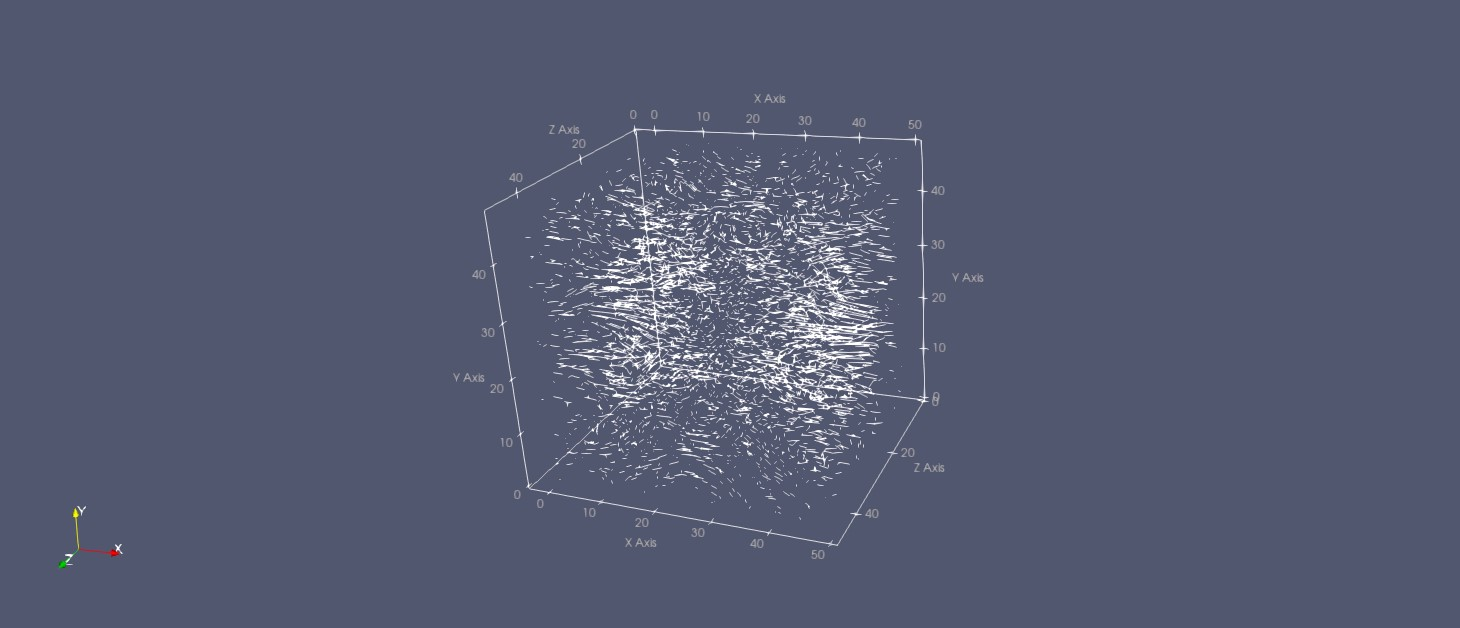
\includegraphics[width=.95\linewidth]{Figures/FDTD3DE4}
		\caption{t = 800}
	\end{subfigure}
	\decoRule
	\caption[3D Electric Field Simulation]{A simulation of the 3D electric field.}
	\label{fig:FDTD3DE}
\end{figure}

\begin{figure}[h!]
	\centering
	\begin{subfigure}{.49\textwidth}
		\centering
		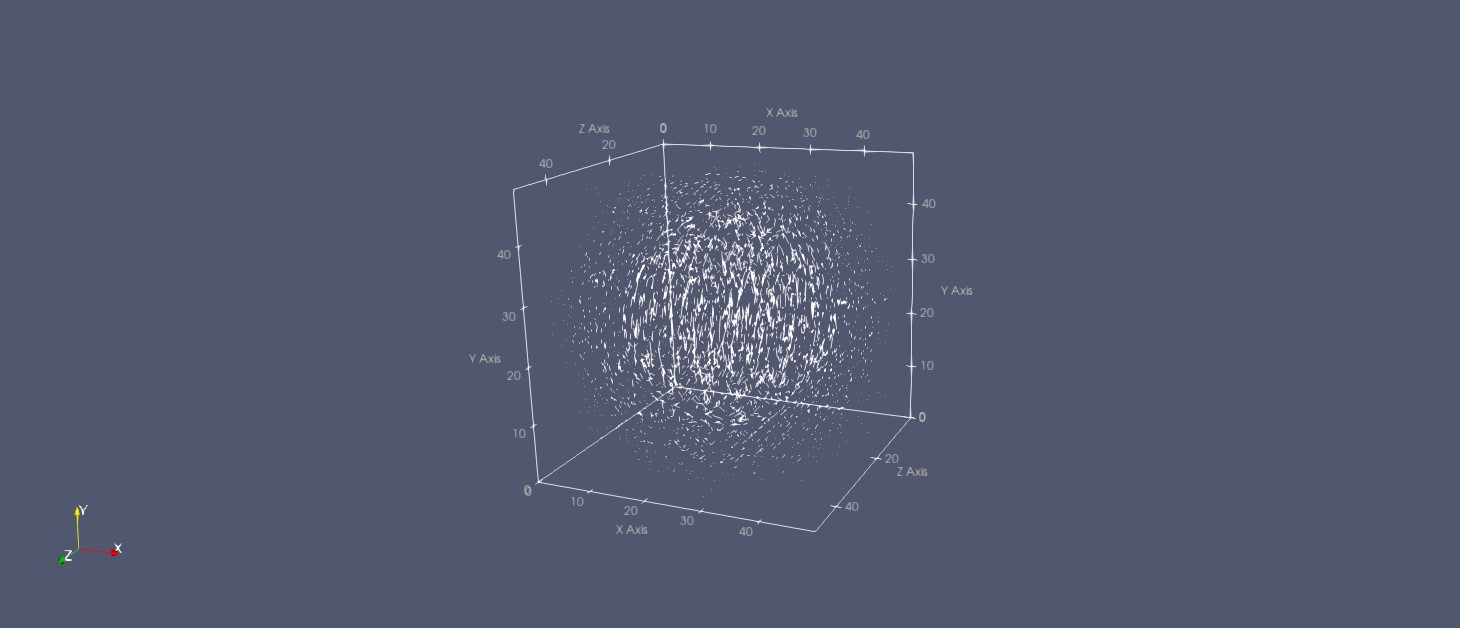
\includegraphics[width=.95\linewidth]{Figures/FDTD3DH1}
		\caption{t = 200}
	\end{subfigure}
	\begin{subfigure}{.49\textwidth}
		\centering
		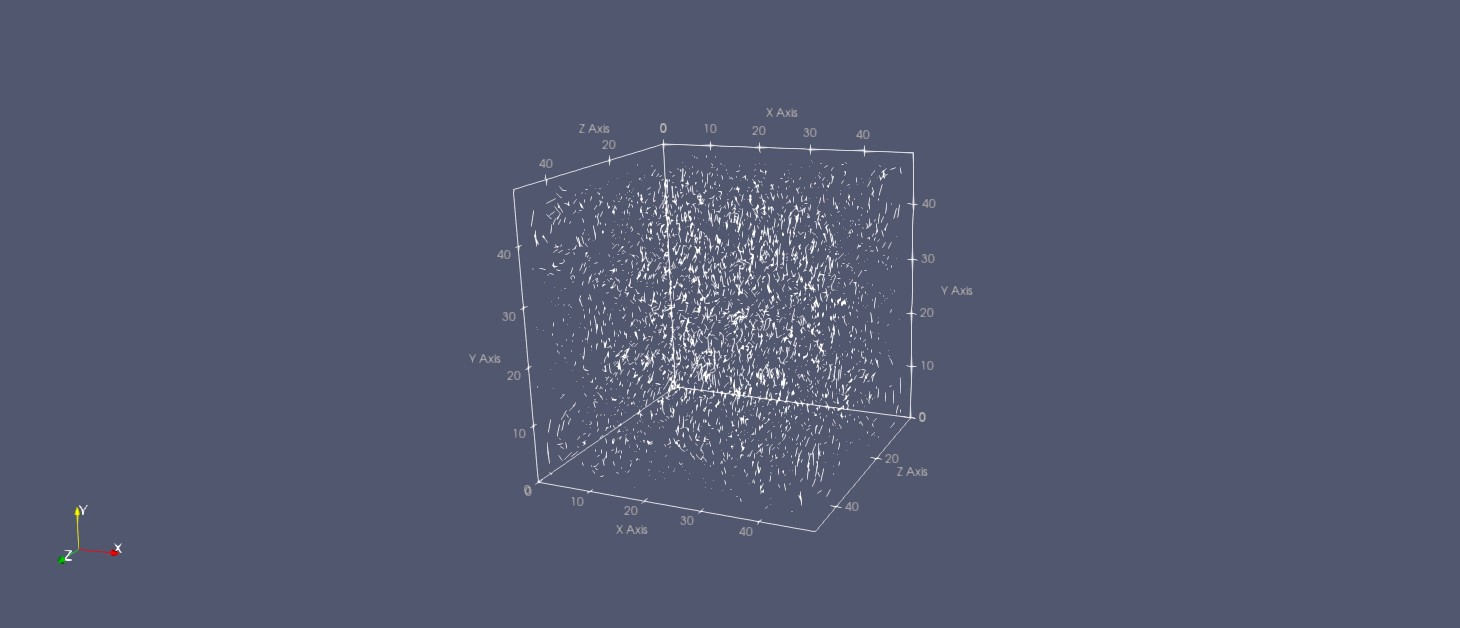
\includegraphics[width=.95\linewidth]{Figures/FDTD3DH2}
		\caption{t = 400}
	\end{subfigure}
	\begin{subfigure}{.49\textwidth}
		\centering
		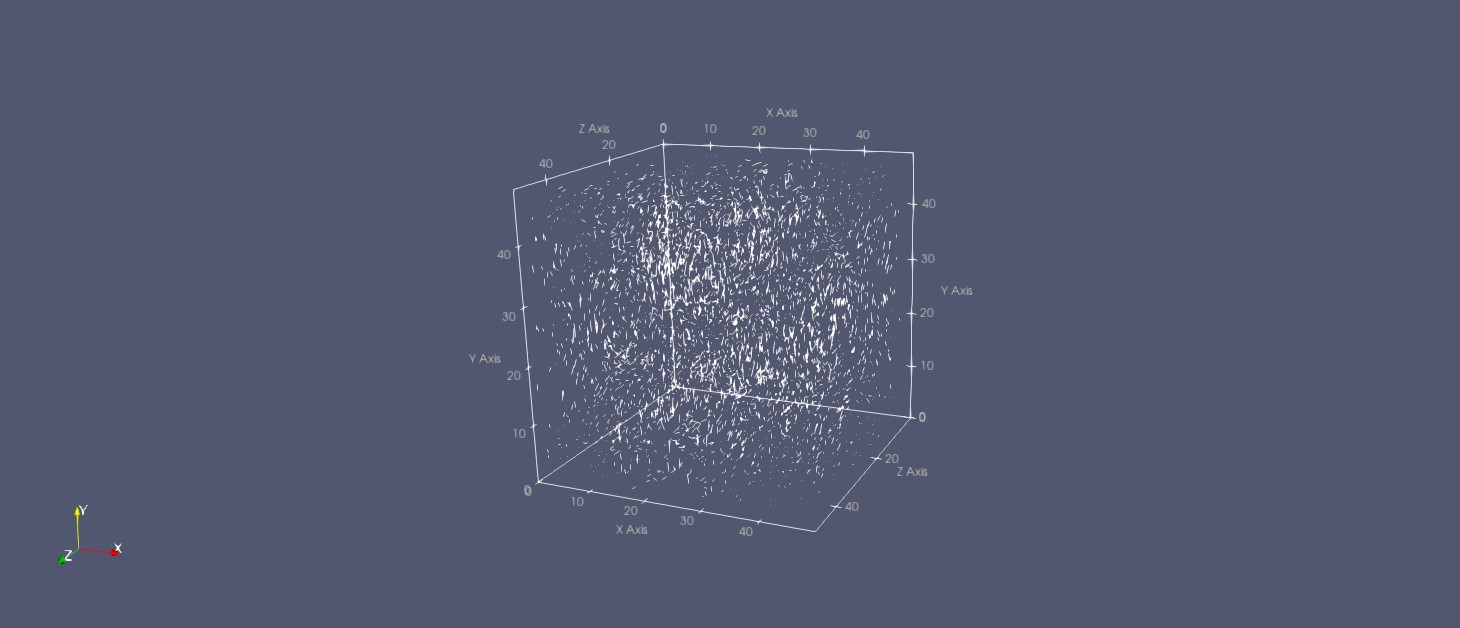
\includegraphics[width=.95\linewidth]{Figures/FDTD3DH3}
		\caption{t = 600}
	\end{subfigure}
	\begin{subfigure}{.49\textwidth}
		\centering
		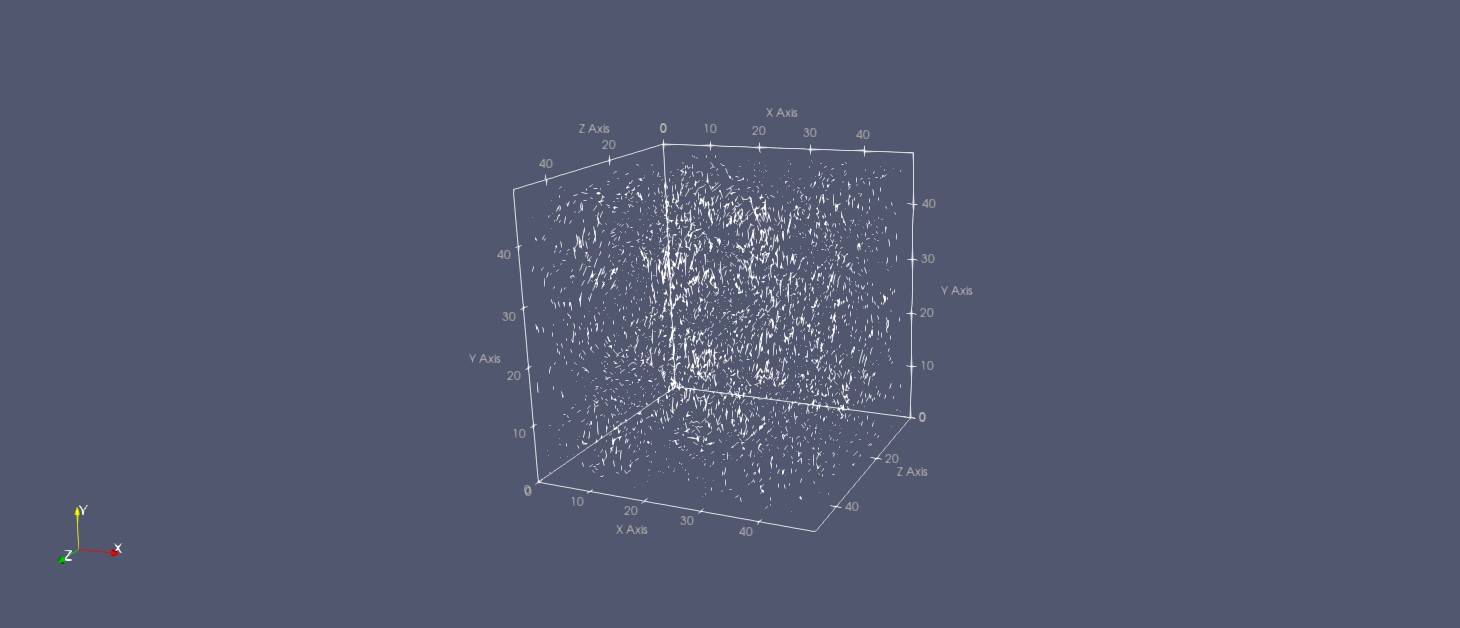
\includegraphics[width=.95\linewidth]{Figures/FDTD3DH4}
		\caption{t = 800}
	\end{subfigure}
	\decoRule
	\caption[3D Magnetic Field Simulation]{A simulation of the 3D magnetic field.}
	\label{fig:FDTD3DH}
\end{figure}